\chapter{Results}
\label{chap:res}
\definecolor{dd_green}{HTML}{00ff00}
\definecolor{dd_red}{HTML}{ff0000}
\definecolor{dd_yellowgreen}{HTML}{88ff00}
\definecolor{dd_yellow}{HTML}{ffff00}
\definecolor{dd_yelloworange}{HTML}{ff8800}
Section \ref{ap:sum} provides a summary of the baseline and results using the {\slshape Global Error} $E^G$ and {\slshape Local Error} $E^L$ metrics. Sections thereafter provide the full baseline and results using the per-joint {\slshape Global Error} $E^G_n$ and {\slshape Local Error} $E^L_n$ metrics. See Section \ref{sec:pm} for details on the performance metrics. The real dataset is the {\slshape MSRA} dataset, and the synthetic datasets are the {\slshape Random MANO} dataset and {\slshape IK MANO} dataset, see Section \ref{sec:sdgm} for details. See Figure \ref{fig:sd:hand} for details on the joint names.

% Good results (around 10 mm) are highlighted in {\bfseries\colorbox{dd_green}{green}}, and bad results (around 100 mm) are highlighted in {\bfseries\colorbox{dd_red}{red}}, results in between (around 50 mm) are defined by appropriate shades of {\bfseries\colorbox{dd_yellow}{yellow}} and {\bfseries\colorbox{dd_yelloworange}{orange}}.

Results are colour-coded, with good results (around 10mm) highlighted in {\bfseries\colorbox{dd_green}{green}}, progressively worse results are highlighted in shades of {\bfseries\colorbox{dd_yellow}{yellow}} and {\bfseries\colorbox{dd_yelloworange}{orange}}, with the worst results highlighted in {\bfseries\colorbox{dd_red}{red}} (> 90mm).
\FloatBarrier\section{Summary}
\label{ap:sum}

\begin{table}[!ht]
    \centering
    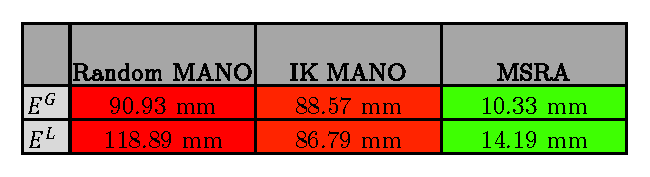
\includegraphics[width=0.7\linewidth]{figs/general/baseline.pdf}
    \caption{The experimental baseline, showing the results when the model is first trained on the MSRA training dataset, then tested on the test MSRA dataset and test synthetic datasets.}
    \end{table}

\begin{table}[!ht]
        \centering
        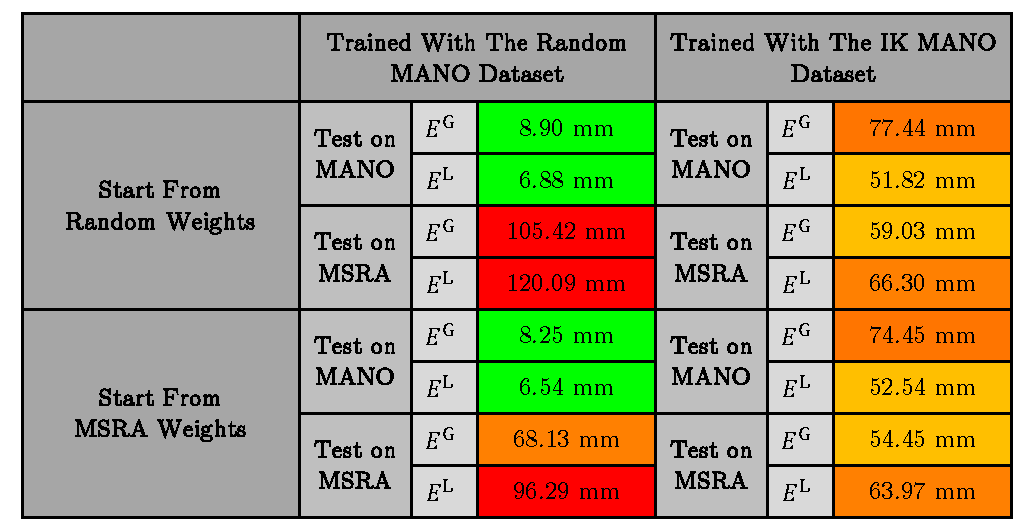
\includegraphics[width=\linewidth]{figs/general/results.pdf}
        \caption{Summary of results over all experiments undertaken. Each experiment reports the average error over all joints for the two metrics described in Section \ref{sec:pm}. See Section \ref{es:exp} for details on the experiments performed.}
    \end{table}


% \FloatBarrier\section{Full Results}
\label{ap:fullres}
\setlength{\tabcolsep}{0.05cm}
\FloatBarrier\section{Baseline Tests}
% All results are in millimeters.
\label{sec:ap:base}
\begin{table}[!ht]
    \begin{tabular}{|c|c|c|c|c|c|c|c|c|c|c|}
    \hline
    \cellcolor[HTML]{40ff00}{\bfseries Wrist} & \cellcolor[HTML]{00ff00}{\bfseries IMCP} & \cellcolor[HTML]{40ff00}{\bfseries IPIP} & \cellcolor[HTML]{40ff00}{\bfseries IDIP} & \cellcolor[HTML]{40ff00}{\bfseries ITIP} & \cellcolor[HTML]{00ff00}{\bfseries MMCP} & \cellcolor[HTML]{00ff00}{\bfseries MPIP} & \cellcolor[HTML]{00ff00}{\bfseries MDIP}  \\
    \cellcolor[HTML]{40ff00}$\,\,\,$10.20 mm & \cellcolor[HTML]{00ff00}$\,\,\,\,\,\,$8.82 mm & \cellcolor[HTML]{40ff00}$\,\,\,$10.10 mm & \cellcolor[HTML]{40ff00}$\,\,\,$10.88 mm & \cellcolor[HTML]{40ff00}$\,\,\,$13.40 mm & \cellcolor[HTML]{00ff00}$\,\,\,\,\,\,$7.33 mm & \cellcolor[HTML]{00ff00}$\,\,\,\,\,\,$8.23 mm & \cellcolor[HTML]{00ff00}$\,\,\,\,\,\,$9.87 mm\\
    \hline
    \cellcolor[HTML]{40ff00}{\bfseries MTIP} & \cellcolor[HTML]{00ff00}{\bfseries RMCP} & \cellcolor[HTML]{00ff00}{\bfseries RPIP} & \cellcolor[HTML]{00ff00}{\bfseries RDIP} & \cellcolor[HTML]{40ff00}{\bfseries RTIP} & \cellcolor[HTML]{00ff00}{\bfseries PMCP} & \cellcolor[HTML]{00ff00}{\bfseries PPIP} & \cellcolor[HTML]{00ff00}{\bfseries PDIP}  \\
    \cellcolor[HTML]{40ff00}$\,\,\,$13.05 mm & \cellcolor[HTML]{00ff00}$\,\,\,\,\,\,$7.56 mm & \cellcolor[HTML]{00ff00}$\,\,\,\,\,\,$7.88 mm & \cellcolor[HTML]{00ff00}$\,\,\,\,\,\,$9.54 mm & \cellcolor[HTML]{40ff00}$\,\,\,$12.68 mm & \cellcolor[HTML]{00ff00}$\,\,\,\,\,\,$9.13 mm & \cellcolor[HTML]{00ff00}$\,\,\,\,\,\,$8.57 mm & \cellcolor[HTML]{00ff00}$\,\,\,\,\,\,$9.27 mm\\
    \hline
    \cellcolor[HTML]{40ff00}{\bfseries PTIP} & \cellcolor[HTML]{00ff00}{\bfseries TMCP} & \cellcolor[HTML]{40ff00}{\bfseries TPIP} & \cellcolor[HTML]{40ff00}{\bfseries PDIP} & \cellcolor[HTML]{40ff00}{\bfseries TTIP} & \cellcolor[HTML]{40ff00}{\bfseries Average}  \\
    \cellcolor[HTML]{40ff00}$\,\,\,$12.04 mm & \cellcolor[HTML]{00ff00}$\,\,\,\,\,\,$9.74 mm & \cellcolor[HTML]{40ff00}$\,\,\,$11.02 mm & \cellcolor[HTML]{40ff00}$\,\,\,$12.00 mm & \cellcolor[HTML]{40ff00}$\,\,\,$15.55 mm & \cellcolor[HTML]{40ff00}$\,\,\,$10.33 mm \\
    \cline{1-6}
    \end{tabular}
    \caption{Global error when model trained with the MSRA dataset initialised with random weights and tested on the MSRA test dataset.}
    \label{tb:baseline_msra:g}
    \end{table}
    \begin{table}[!ht]
    \begin{tabular}{|c|c|c|c|c|c|c|c|c|c|c|}
    \hline
    {\bfseries Wrist} & \cellcolor[HTML]{40ff00}{\bfseries IMCP} & \cellcolor[HTML]{40ff00}{\bfseries IPIP} & \cellcolor[HTML]{40ff00}{\bfseries IDIP} & \cellcolor[HTML]{40ff00}{\bfseries ITIP} & \cellcolor[HTML]{40ff00}{\bfseries MMCP} & \cellcolor[HTML]{40ff00}{\bfseries MPIP} & \cellcolor[HTML]{40ff00}{\bfseries MDIP}  \\
    N/A mm & \cellcolor[HTML]{40ff00}$\,\,\,$10.82 mm & \cellcolor[HTML]{40ff00}$\,\,\,$13.18 mm & \cellcolor[HTML]{40ff00}$\,\,\,$14.75 mm & \cellcolor[HTML]{40ff00}$\,\,\,$17.31 mm & \cellcolor[HTML]{40ff00}$\,\,\,$10.76 mm & \cellcolor[HTML]{40ff00}$\,\,\,$13.45 mm & \cellcolor[HTML]{40ff00}$\,\,\,$15.20 mm\\
    \hline
    \cellcolor[HTML]{40ff00}{\bfseries MTIP} & \cellcolor[HTML]{40ff00}{\bfseries RMCP} & \cellcolor[HTML]{40ff00}{\bfseries RPIP} & \cellcolor[HTML]{40ff00}{\bfseries RDIP} & \cellcolor[HTML]{40ff00}{\bfseries RTIP} & \cellcolor[HTML]{40ff00}{\bfseries PMCP} & \cellcolor[HTML]{40ff00}{\bfseries PPIP} & \cellcolor[HTML]{40ff00}{\bfseries PDIP}  \\
    \cellcolor[HTML]{40ff00}$\,\,\,$17.71 mm & \cellcolor[HTML]{40ff00}$\,\,\,$11.59 mm & \cellcolor[HTML]{40ff00}$\,\,\,$13.63 mm & \cellcolor[HTML]{40ff00}$\,\,\,$15.21 mm & \cellcolor[HTML]{40ff00}$\,\,\,$17.47 mm & \cellcolor[HTML]{40ff00}$\,\,\,$13.20 mm & \cellcolor[HTML]{40ff00}$\,\,\,$13.57 mm & \cellcolor[HTML]{40ff00}$\,\,\,$14.14 mm\\
    \hline
    \cellcolor[HTML]{40ff00}{\bfseries PTIP} & \cellcolor[HTML]{00ff00}{\bfseries TMCP} & \cellcolor[HTML]{40ff00}{\bfseries TPIP} & \cellcolor[HTML]{40ff00}{\bfseries PDIP} & \cellcolor[HTML]{40ff00}{\bfseries TTIP} & \cellcolor[HTML]{40ff00}{\bfseries Average}  \\
    \cellcolor[HTML]{40ff00}$\,\,\,$16.62 mm & \cellcolor[HTML]{00ff00}$\,\,\,\,\,\,$8.72 mm & \cellcolor[HTML]{40ff00}$\,\,\,$12.60 mm & \cellcolor[HTML]{40ff00}$\,\,\,$15.07 mm & \cellcolor[HTML]{40ff00}$\,\,\,$18.86 mm & \cellcolor[HTML]{40ff00}$\,\,\,$14.19 mm \\
    \cline{1-6}
    \end{tabular}
    \caption{Local error when model trained with the MSRA dataset initialised with random weights and tested on the MSRA test dataset.}
    \label{tb:baseline_msra:l}
    \end{table}
\begin{table}[!ht]
    \begin{tabular}{|c|c|c|c|c|c|c|c|c|c|c|}
    \hline
    \cellcolor[HTML]{ff0000}{\bfseries Wrist} & \cellcolor[HTML]{ff0000}{\bfseries IMCP} & \cellcolor[HTML]{ff2500}{\bfseries IPIP} & \cellcolor[HTML]{ff2500}{\bfseries IDIP} & \cellcolor[HTML]{ff2500}{\bfseries ITIP} & \cellcolor[HTML]{ff2500}{\bfseries MMCP} & \cellcolor[HTML]{ff7500}{\bfseries MPIP} & \cellcolor[HTML]{ff7500}{\bfseries MDIP}  \\
    \cellcolor[HTML]{ff0000}123.25 mm & \cellcolor[HTML]{ff0000}105.61 mm & \cellcolor[HTML]{ff2500}$\,\,\,$84.00 mm & \cellcolor[HTML]{ff2500}$\,\,\,$86.13 mm & \cellcolor[HTML]{ff2500}$\,\,\,$84.01 mm & \cellcolor[HTML]{ff2500}$\,\,\,$82.64 mm & \cellcolor[HTML]{ff7500}$\,\,\,$79.98 mm & \cellcolor[HTML]{ff7500}$\,\,\,$70.77 mm\\
    \hline
    \cellcolor[HTML]{ff7500}{\bfseries MTIP} & \cellcolor[HTML]{ff7500}{\bfseries RMCP} & \cellcolor[HTML]{ff7500}{\bfseries RPIP} & \cellcolor[HTML]{ff2500}{\bfseries RDIP} & \cellcolor[HTML]{ff7500}{\bfseries RTIP} & \cellcolor[HTML]{ff2500}{\bfseries PMCP} & \cellcolor[HTML]{ff7500}{\bfseries PPIP} & \cellcolor[HTML]{ff2500}{\bfseries PDIP}  \\
    \cellcolor[HTML]{ff7500}$\,\,\,$72.60 mm & \cellcolor[HTML]{ff7500}$\,\,\,$77.96 mm & \cellcolor[HTML]{ff7500}$\,\,\,$72.01 mm & \cellcolor[HTML]{ff2500}$\,\,\,$81.24 mm & \cellcolor[HTML]{ff7500}$\,\,\,$72.84 mm & \cellcolor[HTML]{ff2500}$\,\,\,$84.75 mm & \cellcolor[HTML]{ff7500}$\,\,\,$79.84 mm & \cellcolor[HTML]{ff2500}$\,\,\,$86.36 mm\\
    \hline
    \cellcolor[HTML]{ff2500}{\bfseries PTIP} & \cellcolor[HTML]{ff0000}{\bfseries TMCP} & \cellcolor[HTML]{ff0000}{\bfseries TPIP} & \cellcolor[HTML]{ff0000}{\bfseries PDIP} & \cellcolor[HTML]{ff0000}{\bfseries TTIP} & \cellcolor[HTML]{ff0000}{\bfseries Average}  \\
    \cellcolor[HTML]{ff2500}$\,\,\,$85.79 mm & \cellcolor[HTML]{ff0000}138.94 mm & \cellcolor[HTML]{ff0000}118.87 mm & \cellcolor[HTML]{ff0000}102.89 mm & \cellcolor[HTML]{ff0000}119.04 mm & \cellcolor[HTML]{ff0000}$\,\,\,$90.93 mm \\
    \cline{1-6}
    \end{tabular}
    \caption{Global error when model trained with the MSRA dataset initialised with random weights and tested on the Random MANO dataset.}
    \label{tb:baseline_mano:g}
    \end{table}
    \begin{table}[!ht]
    \begin{tabular}{|c|c|c|c|c|c|c|c|c|c|c|}
    \hline
    {\bfseries Wrist} & \cellcolor[HTML]{ff0000}{\bfseries IMCP} & \cellcolor[HTML]{ff0000}{\bfseries IPIP} & \cellcolor[HTML]{ff0000}{\bfseries IDIP} & \cellcolor[HTML]{ff0000}{\bfseries ITIP} & \cellcolor[HTML]{ff0000}{\bfseries MMCP} & \cellcolor[HTML]{ff0000}{\bfseries MPIP} & \cellcolor[HTML]{ff0000}{\bfseries MDIP}  \\
    N/A mm & \cellcolor[HTML]{ff0000}121.88 mm & \cellcolor[HTML]{ff0000}117.93 mm & \cellcolor[HTML]{ff0000}127.07 mm & \cellcolor[HTML]{ff0000}130.78 mm & \cellcolor[HTML]{ff0000}115.38 mm & \cellcolor[HTML]{ff0000}113.78 mm & \cellcolor[HTML]{ff0000}109.93 mm\\
    \hline
    \cellcolor[HTML]{ff0000}{\bfseries MTIP} & \cellcolor[HTML]{ff0000}{\bfseries RMCP} & \cellcolor[HTML]{ff0000}{\bfseries RPIP} & \cellcolor[HTML]{ff0000}{\bfseries RDIP} & \cellcolor[HTML]{ff0000}{\bfseries RTIP} & \cellcolor[HTML]{ff0000}{\bfseries PMCP} & \cellcolor[HTML]{ff0000}{\bfseries PPIP} & \cellcolor[HTML]{ff0000}{\bfseries PDIP}  \\
    \cellcolor[HTML]{ff0000}121.37 mm & \cellcolor[HTML]{ff0000}107.26 mm & \cellcolor[HTML]{ff0000}105.41 mm & \cellcolor[HTML]{ff0000}115.54 mm & \cellcolor[HTML]{ff0000}114.41 mm & \cellcolor[HTML]{ff0000}114.18 mm & \cellcolor[HTML]{ff0000}124.42 mm & \cellcolor[HTML]{ff0000}108.09 mm\\
    \hline
    \cellcolor[HTML]{ff0000}{\bfseries PTIP} & \cellcolor[HTML]{ff0000}{\bfseries TMCP} & \cellcolor[HTML]{ff0000}{\bfseries TPIP} & \cellcolor[HTML]{ff0000}{\bfseries PDIP} & \cellcolor[HTML]{ff0000}{\bfseries TTIP} & \cellcolor[HTML]{ff0000}{\bfseries Average}  \\
    \cellcolor[HTML]{ff0000}112.18 mm & \cellcolor[HTML]{ff0000}136.50 mm & \cellcolor[HTML]{ff0000}128.28 mm & \cellcolor[HTML]{ff0000}136.64 mm & \cellcolor[HTML]{ff0000}116.67 mm & \cellcolor[HTML]{ff0000}118.89 mm \\
    \cline{1-6}
    \end{tabular}
    \caption{Local error when model trained with the MSRA dataset initialised with random weights and tested on the Random MANO test dataset.}
    \label{tb:baseline_mano:l}
    \end{table}
\begin{table}[!ht]
    \begin{tabular}{|c|c|c|c|c|c|c|c|c|c|c|}
    \hline
    \cellcolor[HTML]{ff7500}{\bfseries Wrist} & \cellcolor[HTML]{ff7500}{\bfseries IMCP} & \cellcolor[HTML]{ff2500}{\bfseries IPIP} & \cellcolor[HTML]{ff0000}{\bfseries IDIP} & \cellcolor[HTML]{ff0000}{\bfseries ITIP} & \cellcolor[HTML]{ff7500}{\bfseries MMCP} & \cellcolor[HTML]{ff2500}{\bfseries MPIP} & \cellcolor[HTML]{ff0000}{\bfseries MDIP}  \\
    \cellcolor[HTML]{ff7500}$\,\,\,$73.79 mm & \cellcolor[HTML]{ff7500}$\,\,\,$75.54 mm & \cellcolor[HTML]{ff2500}$\,\,\,$86.05 mm & \cellcolor[HTML]{ff0000}$\,\,\,$96.61 mm & \cellcolor[HTML]{ff0000}108.52 mm & \cellcolor[HTML]{ff7500}$\,\,\,$73.57 mm & \cellcolor[HTML]{ff2500}$\,\,\,$89.94 mm & \cellcolor[HTML]{ff0000}100.02 mm\\
    \hline
    \cellcolor[HTML]{ff0000}{\bfseries MTIP} & \cellcolor[HTML]{ff7500}{\bfseries RMCP} & \cellcolor[HTML]{ff2500}{\bfseries RPIP} & \cellcolor[HTML]{ff0000}{\bfseries RDIP} & \cellcolor[HTML]{ff0000}{\bfseries RTIP} & \cellcolor[HTML]{ff7500}{\bfseries PMCP} & \cellcolor[HTML]{ff2500}{\bfseries PPIP} & \cellcolor[HTML]{ff0000}{\bfseries PDIP}  \\
    \cellcolor[HTML]{ff0000}112.83 mm & \cellcolor[HTML]{ff7500}$\,\,\,$75.50 mm & \cellcolor[HTML]{ff2500}$\,\,\,$87.29 mm & \cellcolor[HTML]{ff0000}$\,\,\,$92.89 mm & \cellcolor[HTML]{ff0000}$\,\,\,$98.37 mm & \cellcolor[HTML]{ff7500}$\,\,\,$78.78 mm & \cellcolor[HTML]{ff2500}$\,\,\,$86.27 mm & \cellcolor[HTML]{ff0000}$\,\,\,$92.02 mm\\
    \hline
    \cellcolor[HTML]{ff0000}{\bfseries PTIP} & \cellcolor[HTML]{ff7500}{\bfseries TMCP} & \cellcolor[HTML]{ff7500}{\bfseries TPIP} & \cellcolor[HTML]{ff2500}{\bfseries PDIP} & \cellcolor[HTML]{ff0000}{\bfseries TTIP} & \cellcolor[HTML]{ff2500}{\bfseries Average}  \\
    \cellcolor[HTML]{ff0000}$\,\,\,$98.80 mm & \cellcolor[HTML]{ff7500}$\,\,\,$70.36 mm & \cellcolor[HTML]{ff7500}$\,\,\,$77.56 mm & \cellcolor[HTML]{ff2500}$\,\,\,$85.33 mm & \cellcolor[HTML]{ff0000}$\,\,\,$99.91 mm & \cellcolor[HTML]{ff2500}$\,\,\,$88.57 mm \\
    \cline{1-6}
    \end{tabular}
    \caption{Global error when model trained with the MSRA dataset initialised with random weights and tested on the IK MANO test dataset.}
    \label{tb:baseline_maya:g}
    \end{table}
    \begin{table}[!ht]
    \begin{tabular}{|c|c|c|c|c|c|c|c|c|c|c|}
    \hline
    {\bfseries Wrist} & \cellcolor[HTML]{ff8000}{\bfseries IMCP} & \cellcolor[HTML]{ff2500}{\bfseries IPIP} & \cellcolor[HTML]{ff0000}{\bfseries IDIP} & \cellcolor[HTML]{ff0000}{\bfseries ITIP} & \cellcolor[HTML]{ff8000}{\bfseries MMCP} & \cellcolor[HTML]{ff0000}{\bfseries MPIP} & \cellcolor[HTML]{ff0000}{\bfseries MDIP}  \\
    N/A mm & \cellcolor[HTML]{ff8000}$\,\,\,$67.93 mm & \cellcolor[HTML]{ff2500}$\,\,\,$84.63 mm & \cellcolor[HTML]{ff0000}$\,\,\,$96.64 mm & \cellcolor[HTML]{ff0000}108.02 mm & \cellcolor[HTML]{ff8000}$\,\,\,$69.45 mm & \cellcolor[HTML]{ff0000}$\,\,\,$93.01 mm & \cellcolor[HTML]{ff0000}103.37 mm\\
    \hline
    \cellcolor[HTML]{ff0000}{\bfseries MTIP} & \cellcolor[HTML]{ff7500}{\bfseries RMCP} & \cellcolor[HTML]{ff0000}{\bfseries RPIP} & \cellcolor[HTML]{ff0000}{\bfseries RDIP} & \cellcolor[HTML]{ff0000}{\bfseries RTIP} & \cellcolor[HTML]{ff7500}{\bfseries PMCP} & \cellcolor[HTML]{ff2500}{\bfseries PPIP} & \cellcolor[HTML]{ff0000}{\bfseries PDIP}  \\
    \cellcolor[HTML]{ff0000}115.10 mm & \cellcolor[HTML]{ff7500}$\,\,\,$71.51 mm & \cellcolor[HTML]{ff0000}$\,\,\,$90.29 mm & \cellcolor[HTML]{ff0000}$\,\,\,$96.56 mm & \cellcolor[HTML]{ff0000}100.27 mm & \cellcolor[HTML]{ff7500}$\,\,\,$75.71 mm & \cellcolor[HTML]{ff2500}$\,\,\,$88.43 mm & \cellcolor[HTML]{ff0000}$\,\,\,$94.82 mm\\
    \hline
    \cellcolor[HTML]{ff0000}{\bfseries PTIP} & \cellcolor[HTML]{ffff00}{\bfseries TMCP} & \cellcolor[HTML]{ff8000}{\bfseries TPIP} & \cellcolor[HTML]{ff7500}{\bfseries PDIP} & \cellcolor[HTML]{ff0000}{\bfseries TTIP} & \cellcolor[HTML]{ff2500}{\bfseries Average}  \\
    \cellcolor[HTML]{ff0000}101.63 mm & \cellcolor[HTML]{ffff00}$\,\,\,$42.45 mm & \cellcolor[HTML]{ff8000}$\,\,\,$64.63 mm & \cellcolor[HTML]{ff7500}$\,\,\,$77.68 mm & \cellcolor[HTML]{ff0000}$\,\,\,$93.73 mm & \cellcolor[HTML]{ff2500}$\,\,\,$86.79 mm \\
    \cline{1-6}
    \end{tabular}
    \caption{Local error when model trained with the MSRA dataset initialised with random weights and tested on the IK MANO test dataset.}
    \label{tb:baseline_maya:l}
    \end{table}

\FloatBarrier\section{Training With The Random MANO Synthetic Dataset}
% All results are in millimeters.
\label{sec:ap:mano}
\begin{table}[!ht]
    \begin{tabular}{|c|c|c|c|c|c|c|c|c|c|c|}
    \hline
    \cellcolor[HTML]{00ff00}{\bfseries Wrist} & \cellcolor[HTML]{00ff00}{\bfseries IMCP} & \cellcolor[HTML]{00ff00}{\bfseries IPIP} & \cellcolor[HTML]{00ff00}{\bfseries IDIP} & \cellcolor[HTML]{40ff00}{\bfseries ITIP} & \cellcolor[HTML]{00ff00}{\bfseries MMCP} & \cellcolor[HTML]{00ff00}{\bfseries MPIP} & \cellcolor[HTML]{00ff00}{\bfseries MDIP}  \\
    \cellcolor[HTML]{00ff00}$\,\,\,\,\,\,$8.39 mm & \cellcolor[HTML]{00ff00}$\,\,\,\,\,\,$8.30 mm & \cellcolor[HTML]{00ff00}$\,\,\,\,\,\,$8.68 mm & \cellcolor[HTML]{00ff00}$\,\,\,\,\,\,$9.48 mm & \cellcolor[HTML]{40ff00}$\,\,\,$11.10 mm & \cellcolor[HTML]{00ff00}$\,\,\,\,\,\,$7.70 mm & \cellcolor[HTML]{00ff00}$\,\,\,\,\,\,$7.90 mm & \cellcolor[HTML]{00ff00}$\,\,\,\,\,\,$8.35 mm\\
    \hline
    \cellcolor[HTML]{00ff00}{\bfseries MTIP} & \cellcolor[HTML]{00ff00}{\bfseries RMCP} & \cellcolor[HTML]{00ff00}{\bfseries RPIP} & \cellcolor[HTML]{00ff00}{\bfseries RDIP} & \cellcolor[HTML]{40ff00}{\bfseries RTIP} & \cellcolor[HTML]{00ff00}{\bfseries PMCP} & \cellcolor[HTML]{00ff00}{\bfseries PPIP} & \cellcolor[HTML]{00ff00}{\bfseries PDIP}  \\
    \cellcolor[HTML]{00ff00}$\,\,\,\,\,\,$9.97 mm & \cellcolor[HTML]{00ff00}$\,\,\,\,\,\,$7.28 mm & \cellcolor[HTML]{00ff00}$\,\,\,\,\,\,$7.54 mm & \cellcolor[HTML]{00ff00}$\,\,\,\,\,\,$8.29 mm & \cellcolor[HTML]{40ff00}$\,\,\,$10.46 mm & \cellcolor[HTML]{00ff00}$\,\,\,\,\,\,$7.25 mm & \cellcolor[HTML]{00ff00}$\,\,\,\,\,\,$7.73 mm & \cellcolor[HTML]{00ff00}$\,\,\,\,\,\,$8.75 mm\\
    \hline
    \cellcolor[HTML]{40ff00}{\bfseries PTIP} & \cellcolor[HTML]{00ff00}{\bfseries TMCP} & \cellcolor[HTML]{00ff00}{\bfseries TPIP} & \cellcolor[HTML]{00ff00}{\bfseries PDIP} & \cellcolor[HTML]{40ff00}{\bfseries TTIP} & \cellcolor[HTML]{00ff00}{\bfseries Average}  \\
    \cellcolor[HTML]{40ff00}$\,\,\,$10.97 mm & \cellcolor[HTML]{00ff00}$\,\,\,\,\,\,$8.29 mm & \cellcolor[HTML]{00ff00}$\,\,\,\,\,\,$8.65 mm & \cellcolor[HTML]{00ff00}$\,\,\,\,\,\,$9.68 mm & \cellcolor[HTML]{40ff00}$\,\,\,$12.12 mm & \cellcolor[HTML]{00ff00}$\,\,\,\,\,\,$8.90 mm \\
    \cline{1-6}
    \end{tabular}
    \caption{Global error when model trained with Random MANO dataset initialised with random weights and tested on Random MANO test dataset.}
    \label{tb:orog}
    \end{table}
    \begin{table}[!ht]
    \begin{tabular}{|c|c|c|c|c|c|c|c|c|c|c|}
    \hline
    {\bfseries Wrist} & \cellcolor[HTML]{00ff00}{\bfseries IMCP} & \cellcolor[HTML]{00ff00}{\bfseries IPIP} & \cellcolor[HTML]{00ff00}{\bfseries IDIP} & \cellcolor[HTML]{00ff00}{\bfseries ITIP} & \cellcolor[HTML]{00ff00}{\bfseries MMCP} & \cellcolor[HTML]{00ff00}{\bfseries MPIP} & \cellcolor[HTML]{00ff00}{\bfseries MDIP}  \\
    N/A mm & \cellcolor[HTML]{00ff00}$\,\,\,\,\,\,$5.08 mm & \cellcolor[HTML]{00ff00}$\,\,\,\,\,\,$6.13 mm & \cellcolor[HTML]{00ff00}$\,\,\,\,\,\,$7.41 mm & \cellcolor[HTML]{00ff00}$\,\,\,\,\,\,$9.74 mm & \cellcolor[HTML]{00ff00}$\,\,\,\,\,\,$4.84 mm & \cellcolor[HTML]{00ff00}$\,\,\,\,\,\,$5.89 mm & \cellcolor[HTML]{00ff00}$\,\,\,\,\,\,$6.93 mm\\
    \hline
    \cellcolor[HTML]{00ff00}{\bfseries MTIP} & \cellcolor[HTML]{00ff00}{\bfseries RMCP} & \cellcolor[HTML]{00ff00}{\bfseries RPIP} & \cellcolor[HTML]{00ff00}{\bfseries RDIP} & \cellcolor[HTML]{00ff00}{\bfseries RTIP} & \cellcolor[HTML]{00ff00}{\bfseries PMCP} & \cellcolor[HTML]{00ff00}{\bfseries PPIP} & \cellcolor[HTML]{00ff00}{\bfseries PDIP}  \\
    \cellcolor[HTML]{00ff00}$\,\,\,\,\,\,$9.16 mm & \cellcolor[HTML]{00ff00}$\,\,\,\,\,\,$4.68 mm & \cellcolor[HTML]{00ff00}$\,\,\,\,\,\,$5.69 mm & \cellcolor[HTML]{00ff00}$\,\,\,\,\,\,$7.09 mm & \cellcolor[HTML]{00ff00}$\,\,\,\,\,\,$9.87 mm & \cellcolor[HTML]{00ff00}$\,\,\,\,\,\,$4.89 mm & \cellcolor[HTML]{00ff00}$\,\,\,\,\,\,$6.03 mm & \cellcolor[HTML]{00ff00}$\,\,\,\,\,\,$7.56 mm\\
    \hline
    \cellcolor[HTML]{40ff00}{\bfseries PTIP} & \cellcolor[HTML]{00ff00}{\bfseries TMCP} & \cellcolor[HTML]{00ff00}{\bfseries TPIP} & \cellcolor[HTML]{00ff00}{\bfseries PDIP} & \cellcolor[HTML]{40ff00}{\bfseries TTIP} & \cellcolor[HTML]{00ff00}{\bfseries Average}  \\
    \cellcolor[HTML]{40ff00}$\,\,\,$10.23 mm & \cellcolor[HTML]{00ff00}$\,\,\,\,\,\,$3.95 mm & \cellcolor[HTML]{00ff00}$\,\,\,\,\,\,$5.08 mm & \cellcolor[HTML]{00ff00}$\,\,\,\,\,\,$6.89 mm & \cellcolor[HTML]{40ff00}$\,\,\,$10.37 mm & \cellcolor[HTML]{00ff00}$\,\,\,\,\,\,$6.88 mm \\
    \cline{1-6}
    \end{tabular}
    \caption{Local error when model trained with Random MANO dataset initialised with random weights and tested on Random MANO test dataset.}
    \label{tb:orol}
    \end{table}
\begin{table}[!ht]
    \begin{tabular}{|c|c|c|c|c|c|c|c|c|c|c|}
    \hline
    \cellcolor[HTML]{ff7500}{\bfseries Wrist} & \cellcolor[HTML]{ff0000}{\bfseries IMCP} & \cellcolor[HTML]{ff0000}{\bfseries IPIP} & \cellcolor[HTML]{ff0000}{\bfseries IDIP} & \cellcolor[HTML]{ff0000}{\bfseries ITIP} & \cellcolor[HTML]{ff0000}{\bfseries MMCP} & \cellcolor[HTML]{ff0000}{\bfseries MPIP} & \cellcolor[HTML]{ff0000}{\bfseries MDIP}  \\
    \cellcolor[HTML]{ff7500}$\,\,\,$75.91 mm & \cellcolor[HTML]{ff0000}$\,\,\,$99.64 mm & \cellcolor[HTML]{ff0000}108.10 mm & \cellcolor[HTML]{ff0000}106.09 mm & \cellcolor[HTML]{ff0000}108.97 mm & \cellcolor[HTML]{ff0000}109.41 mm & \cellcolor[HTML]{ff0000}104.96 mm & \cellcolor[HTML]{ff0000}105.99 mm\\
    \hline
    \cellcolor[HTML]{ff0000}{\bfseries MTIP} & \cellcolor[HTML]{ff0000}{\bfseries RMCP} & \cellcolor[HTML]{ff0000}{\bfseries RPIP} & \cellcolor[HTML]{ff0000}{\bfseries RDIP} & \cellcolor[HTML]{ff0000}{\bfseries RTIP} & \cellcolor[HTML]{ff0000}{\bfseries PMCP} & \cellcolor[HTML]{ff0000}{\bfseries PPIP} & \cellcolor[HTML]{ff0000}{\bfseries PDIP}  \\
    \cellcolor[HTML]{ff0000}110.81 mm & \cellcolor[HTML]{ff0000}110.22 mm & \cellcolor[HTML]{ff0000}106.17 mm & \cellcolor[HTML]{ff0000}107.01 mm & \cellcolor[HTML]{ff0000}107.00 mm & \cellcolor[HTML]{ff0000}103.82 mm & \cellcolor[HTML]{ff0000}111.16 mm & \cellcolor[HTML]{ff0000}112.72 mm\\
    \hline
    \cellcolor[HTML]{ff0000}{\bfseries PTIP} & \cellcolor[HTML]{ff2500}{\bfseries TMCP} & \cellcolor[HTML]{ff0000}{\bfseries TPIP} & \cellcolor[HTML]{ff0000}{\bfseries PDIP} & \cellcolor[HTML]{ff0000}{\bfseries TTIP} & \cellcolor[HTML]{ff0000}{\bfseries Average}  \\
    \cellcolor[HTML]{ff0000}111.82 mm & \cellcolor[HTML]{ff2500}$\,\,\,$85.61 mm & \cellcolor[HTML]{ff0000}101.98 mm & \cellcolor[HTML]{ff0000}112.97 mm & \cellcolor[HTML]{ff0000}113.48 mm & \cellcolor[HTML]{ff0000}105.42 mm \\
    \cline{1-6}
    \end{tabular}
    \caption{Global error when model trained with Random MANO dataset initialised with random weights and tested on MSRA test dataset.}
    \label{tb:orag}
    \end{table}
    \begin{table}[!ht]
    \begin{tabular}{|c|c|c|c|c|c|c|c|c|c|c|}
    \hline
    {\bfseries Wrist} & \cellcolor[HTML]{ff0000}{\bfseries IMCP} & \cellcolor[HTML]{ff0000}{\bfseries IPIP} & \cellcolor[HTML]{ff0000}{\bfseries IDIP} & \cellcolor[HTML]{ff0000}{\bfseries ITIP} & \cellcolor[HTML]{ff0000}{\bfseries MMCP} & \cellcolor[HTML]{ff0000}{\bfseries MPIP} & \cellcolor[HTML]{ff0000}{\bfseries MDIP}  \\
    N/A mm & \cellcolor[HTML]{ff0000}109.93 mm & \cellcolor[HTML]{ff0000}121.02 mm & \cellcolor[HTML]{ff0000}120.88 mm & \cellcolor[HTML]{ff0000}126.14 mm & \cellcolor[HTML]{ff0000}121.30 mm & \cellcolor[HTML]{ff0000}126.35 mm & \cellcolor[HTML]{ff0000}126.83 mm\\
    \hline
    \cellcolor[HTML]{ff0000}{\bfseries MTIP} & \cellcolor[HTML]{ff0000}{\bfseries RMCP} & \cellcolor[HTML]{ff0000}{\bfseries RPIP} & \cellcolor[HTML]{ff0000}{\bfseries RDIP} & \cellcolor[HTML]{ff0000}{\bfseries RTIP} & \cellcolor[HTML]{ff0000}{\bfseries PMCP} & \cellcolor[HTML]{ff0000}{\bfseries PPIP} & \cellcolor[HTML]{ff0000}{\bfseries PDIP}  \\
    \cellcolor[HTML]{ff0000}130.08 mm & \cellcolor[HTML]{ff0000}123.69 mm & \cellcolor[HTML]{ff0000}128.24 mm & \cellcolor[HTML]{ff0000}127.39 mm & \cellcolor[HTML]{ff0000}125.41 mm & \cellcolor[HTML]{ff0000}117.20 mm & \cellcolor[HTML]{ff0000}130.32 mm & \cellcolor[HTML]{ff0000}133.18 mm\\
    \hline
    \cellcolor[HTML]{ff0000}{\bfseries PTIP} & \cellcolor[HTML]{ff8000}{\bfseries TMCP} & \cellcolor[HTML]{ff0000}{\bfseries TPIP} & \cellcolor[HTML]{ff0000}{\bfseries PDIP} & \cellcolor[HTML]{ff0000}{\bfseries TTIP} & \cellcolor[HTML]{ff0000}{\bfseries Average}  \\
    \cellcolor[HTML]{ff0000}133.56 mm & \cellcolor[HTML]{ff8000}$\,\,\,$68.03 mm & \cellcolor[HTML]{ff0000}$\,\,\,$99.87 mm & \cellcolor[HTML]{ff0000}114.25 mm & \cellcolor[HTML]{ff0000}118.20 mm & \cellcolor[HTML]{ff0000}120.09 mm \\
    \cline{1-6}
    \end{tabular}
    \caption{Local error when model trained with Random MANO dataset initialised with random weights and tested on MSRA test dataset.}
    \label{tb:oral}
    \end{table}
\begin{table}[!ht]
    \begin{tabular}{|c|c|c|c|c|c|c|c|c|c|c|}
    \hline
    \cellcolor[HTML]{00ff00}{\bfseries Wrist} & \cellcolor[HTML]{00ff00}{\bfseries IMCP} & \cellcolor[HTML]{00ff00}{\bfseries IPIP} & \cellcolor[HTML]{00ff00}{\bfseries IDIP} & \cellcolor[HTML]{40ff00}{\bfseries ITIP} & \cellcolor[HTML]{00ff00}{\bfseries MMCP} & \cellcolor[HTML]{00ff00}{\bfseries MPIP} & \cellcolor[HTML]{00ff00}{\bfseries MDIP}  \\
    \cellcolor[HTML]{00ff00}$\,\,\,\,\,\,$7.77 mm & \cellcolor[HTML]{00ff00}$\,\,\,\,\,\,$7.45 mm & \cellcolor[HTML]{00ff00}$\,\,\,\,\,\,$7.79 mm & \cellcolor[HTML]{00ff00}$\,\,\,\,\,\,$8.70 mm & \cellcolor[HTML]{40ff00}$\,\,\,$10.49 mm & \cellcolor[HTML]{00ff00}$\,\,\,\,\,\,$6.88 mm & \cellcolor[HTML]{00ff00}$\,\,\,\,\,\,$7.23 mm & \cellcolor[HTML]{00ff00}$\,\,\,\,\,\,$7.94 mm\\
    \hline
    \cellcolor[HTML]{00ff00}{\bfseries MTIP} & \cellcolor[HTML]{00ff00}{\bfseries RMCP} & \cellcolor[HTML]{00ff00}{\bfseries RPIP} & \cellcolor[HTML]{00ff00}{\bfseries RDIP} & \cellcolor[HTML]{00ff00}{\bfseries RTIP} & \cellcolor[HTML]{00ff00}{\bfseries PMCP} & \cellcolor[HTML]{00ff00}{\bfseries PPIP} & \cellcolor[HTML]{00ff00}{\bfseries PDIP}  \\
    \cellcolor[HTML]{00ff00}$\,\,\,\,\,\,$9.75 mm & \cellcolor[HTML]{00ff00}$\,\,\,\,\,\,$6.66 mm & \cellcolor[HTML]{00ff00}$\,\,\,\,\,\,$6.82 mm & \cellcolor[HTML]{00ff00}$\,\,\,\,\,\,$7.76 mm & \cellcolor[HTML]{00ff00}$\,\,\,\,\,\,$9.87 mm & \cellcolor[HTML]{00ff00}$\,\,\,\,\,\,$6.61 mm & \cellcolor[HTML]{00ff00}$\,\,\,\,\,\,$7.05 mm & \cellcolor[HTML]{00ff00}$\,\,\,\,\,\,$8.12 mm\\
    \hline
    \cellcolor[HTML]{40ff00}{\bfseries PTIP} & \cellcolor[HTML]{00ff00}{\bfseries TMCP} & \cellcolor[HTML]{00ff00}{\bfseries TPIP} & \cellcolor[HTML]{00ff00}{\bfseries PDIP} & \cellcolor[HTML]{40ff00}{\bfseries TTIP} & \cellcolor[HTML]{00ff00}{\bfseries Average}  \\
    \cellcolor[HTML]{40ff00}$\,\,\,$10.19 mm & \cellcolor[HTML]{00ff00}$\,\,\,\,\,\,$7.79 mm & \cellcolor[HTML]{00ff00}$\,\,\,\,\,\,$7.96 mm & \cellcolor[HTML]{00ff00}$\,\,\,\,\,\,$9.12 mm & \cellcolor[HTML]{40ff00}$\,\,\,$11.29 mm & \cellcolor[HTML]{00ff00}$\,\,\,\,\,\,$8.25 mm \\
    \cline{1-6}
    \end{tabular}
    \caption{Local error when model trained with Random MANO dataset initialised with MSRA weights and tested on Random MANO test dataset.}
    \label{tb:omog}
    \end{table}
    \begin{table}[!ht]
    \begin{tabular}{|c|c|c|c|c|c|c|c|c|c|c|}
    \hline
    {\bfseries Wrist} & \cellcolor[HTML]{00ff00}{\bfseries IMCP} & \cellcolor[HTML]{00ff00}{\bfseries IPIP} & \cellcolor[HTML]{00ff00}{\bfseries IDIP} & \cellcolor[HTML]{00ff00}{\bfseries ITIP} & \cellcolor[HTML]{00ff00}{\bfseries MMCP} & \cellcolor[HTML]{00ff00}{\bfseries MPIP} & \cellcolor[HTML]{00ff00}{\bfseries MDIP}  \\
    N/A mm & \cellcolor[HTML]{00ff00}$\,\,\,\,\,\,$4.84 mm & \cellcolor[HTML]{00ff00}$\,\,\,\,\,\,$5.72 mm & \cellcolor[HTML]{00ff00}$\,\,\,\,\,\,$6.90 mm & \cellcolor[HTML]{00ff00}$\,\,\,\,\,\,$8.98 mm & \cellcolor[HTML]{00ff00}$\,\,\,\,\,\,$4.73 mm & \cellcolor[HTML]{00ff00}$\,\,\,\,\,\,$5.66 mm & \cellcolor[HTML]{00ff00}$\,\,\,\,\,\,$6.72 mm\\
    \hline
    \cellcolor[HTML]{00ff00}{\bfseries MTIP} & \cellcolor[HTML]{00ff00}{\bfseries RMCP} & \cellcolor[HTML]{00ff00}{\bfseries RPIP} & \cellcolor[HTML]{00ff00}{\bfseries RDIP} & \cellcolor[HTML]{00ff00}{\bfseries RTIP} & \cellcolor[HTML]{00ff00}{\bfseries PMCP} & \cellcolor[HTML]{00ff00}{\bfseries PPIP} & \cellcolor[HTML]{00ff00}{\bfseries PDIP}  \\
    \cellcolor[HTML]{00ff00}$\,\,\,\,\,\,$8.84 mm & \cellcolor[HTML]{00ff00}$\,\,\,\,\,\,$4.50 mm & \cellcolor[HTML]{00ff00}$\,\,\,\,\,\,$5.39 mm & \cellcolor[HTML]{00ff00}$\,\,\,\,\,\,$6.70 mm & \cellcolor[HTML]{00ff00}$\,\,\,\,\,\,$9.18 mm & \cellcolor[HTML]{00ff00}$\,\,\,\,\,\,$4.60 mm & \cellcolor[HTML]{00ff00}$\,\,\,\,\,\,$5.61 mm & \cellcolor[HTML]{00ff00}$\,\,\,\,\,\,$7.10 mm\\
    \hline
    \cellcolor[HTML]{00ff00}{\bfseries PTIP} & \cellcolor[HTML]{00ff00}{\bfseries TMCP} & \cellcolor[HTML]{00ff00}{\bfseries TPIP} & \cellcolor[HTML]{00ff00}{\bfseries PDIP} & \cellcolor[HTML]{00ff00}{\bfseries TTIP} & \cellcolor[HTML]{00ff00}{\bfseries Average}  \\
    \cellcolor[HTML]{00ff00}$\,\,\,\,\,\,$9.53 mm & \cellcolor[HTML]{00ff00}$\,\,\,\,\,\,$3.94 mm & \cellcolor[HTML]{00ff00}$\,\,\,\,\,\,$4.97 mm & \cellcolor[HTML]{00ff00}$\,\,\,\,\,\,$6.97 mm & \cellcolor[HTML]{00ff00}$\,\,\,\,\,\,$9.92 mm & \cellcolor[HTML]{00ff00}$\,\,\,\,\,\,$6.54 mm \\
    \cline{1-6}
    \end{tabular}
    \caption{Local error when model trained with Random MANO dataset initialised with MSRA weights and tested on Random MANO test dataset.}
    \label{tb:omol}
    \end{table}
\begin{table}[!ht]
    \begin{tabular}{|c|c|c|c|c|c|c|c|c|c|c|}
    \hline
    \cellcolor[HTML]{ff8000}{\bfseries Wrist} & \cellcolor[HTML]{ffbf00}{\bfseries IMCP} & \cellcolor[HTML]{ff2500}{\bfseries IPIP} & \cellcolor[HTML]{ff0000}{\bfseries IDIP} & \cellcolor[HTML]{ff0000}{\bfseries ITIP} & \cellcolor[HTML]{ffbf00}{\bfseries MMCP} & \cellcolor[HTML]{ff7500}{\bfseries MPIP} & \cellcolor[HTML]{ff7500}{\bfseries MDIP}  \\
    \cellcolor[HTML]{ff8000}$\,\,\,$66.27 mm & \cellcolor[HTML]{ffbf00}$\,\,\,$56.85 mm & \cellcolor[HTML]{ff2500}$\,\,\,$81.36 mm & \cellcolor[HTML]{ff0000}$\,\,\,$94.68 mm & \cellcolor[HTML]{ff0000}$\,\,\,$92.93 mm & \cellcolor[HTML]{ffbf00}$\,\,\,$52.51 mm & \cellcolor[HTML]{ff7500}$\,\,\,$74.99 mm & \cellcolor[HTML]{ff7500}$\,\,\,$79.10 mm\\
    \hline
    \cellcolor[HTML]{ff7500}{\bfseries MTIP} & \cellcolor[HTML]{ffff00}{\bfseries RMCP} & \cellcolor[HTML]{ffbf00}{\bfseries RPIP} & \cellcolor[HTML]{ff8000}{\bfseries RDIP} & \cellcolor[HTML]{ff8000}{\bfseries RTIP} & \cellcolor[HTML]{ffbf00}{\bfseries PMCP} & \cellcolor[HTML]{ff8000}{\bfseries PPIP} & \cellcolor[HTML]{ff7500}{\bfseries PDIP}  \\
    \cellcolor[HTML]{ff7500}$\,\,\,$79.83 mm & \cellcolor[HTML]{ffff00}$\,\,\,$48.45 mm & \cellcolor[HTML]{ffbf00}$\,\,\,$57.67 mm & \cellcolor[HTML]{ff8000}$\,\,\,$63.70 mm & \cellcolor[HTML]{ff8000}$\,\,\,$64.44 mm & \cellcolor[HTML]{ffbf00}$\,\,\,$57.67 mm & \cellcolor[HTML]{ff8000}$\,\,\,$68.19 mm & \cellcolor[HTML]{ff7500}$\,\,\,$72.50 mm\\
    \hline
    \cellcolor[HTML]{ff7500}{\bfseries PTIP} & \cellcolor[HTML]{ffff00}{\bfseries TMCP} & \cellcolor[HTML]{ffff00}{\bfseries TPIP} & \cellcolor[HTML]{ff8000}{\bfseries PDIP} & \cellcolor[HTML]{ff2500}{\bfseries TTIP} & \cellcolor[HTML]{ff8000}{\bfseries Average}  \\
    \cellcolor[HTML]{ff7500}$\,\,\,$75.13 mm & \cellcolor[HTML]{ffff00}$\,\,\,$45.56 mm & \cellcolor[HTML]{ffff00}$\,\,\,$48.79 mm & \cellcolor[HTML]{ff8000}$\,\,\,$66.76 mm & \cellcolor[HTML]{ff2500}$\,\,\,$83.37 mm & \cellcolor[HTML]{ff8000}$\,\,\,$68.13 mm \\
    \cline{1-6}
    \end{tabular}
    \caption{Global error when model trained with Random MANO dataset initialised with MSRA weights and tested on MSRA test dataset.}
    \label{tb:omag}
    \end{table}
    \begin{table}[!ht]
    \begin{tabular}{|c|c|c|c|c|c|c|c|c|c|c|}
    \hline
    {\bfseries Wrist} & \cellcolor[HTML]{ff2500}{\bfseries IMCP} & \cellcolor[HTML]{ff0000}{\bfseries IPIP} & \cellcolor[HTML]{ff0000}{\bfseries IDIP} & \cellcolor[HTML]{ff0000}{\bfseries ITIP} & \cellcolor[HTML]{ff2500}{\bfseries MMCP} & \cellcolor[HTML]{ff0000}{\bfseries MPIP} & \cellcolor[HTML]{ff0000}{\bfseries MDIP}  \\
    N/A mm & \cellcolor[HTML]{ff2500}$\,\,\,$83.09 mm & \cellcolor[HTML]{ff0000}103.47 mm & \cellcolor[HTML]{ff0000}117.67 mm & \cellcolor[HTML]{ff0000}119.24 mm & \cellcolor[HTML]{ff2500}$\,\,\,$83.72 mm & \cellcolor[HTML]{ff0000}106.87 mm & \cellcolor[HTML]{ff0000}110.43 mm\\
    \hline
    \cellcolor[HTML]{ff0000}{\bfseries MTIP} & \cellcolor[HTML]{ff2500}{\bfseries RMCP} & \cellcolor[HTML]{ff0000}{\bfseries RPIP} & \cellcolor[HTML]{ff0000}{\bfseries RDIP} & \cellcolor[HTML]{ff0000}{\bfseries RTIP} & \cellcolor[HTML]{ff2500}{\bfseries PMCP} & \cellcolor[HTML]{ff0000}{\bfseries PPIP} & \cellcolor[HTML]{ff0000}{\bfseries PDIP}  \\
    \cellcolor[HTML]{ff0000}109.72 mm & \cellcolor[HTML]{ff2500}$\,\,\,$83.35 mm & \cellcolor[HTML]{ff0000}$\,\,\,$94.33 mm & \cellcolor[HTML]{ff0000}$\,\,\,$98.46 mm & \cellcolor[HTML]{ff0000}$\,\,\,$98.78 mm & \cellcolor[HTML]{ff2500}$\,\,\,$87.96 mm & \cellcolor[HTML]{ff0000}$\,\,\,$97.24 mm & \cellcolor[HTML]{ff0000}102.23 mm\\
    \hline
    \cellcolor[HTML]{ff0000}{\bfseries PTIP} & \cellcolor[HTML]{ffbf00}{\bfseries TMCP} & \cellcolor[HTML]{ff7500}{\bfseries TPIP} & \cellcolor[HTML]{ff2500}{\bfseries PDIP} & \cellcolor[HTML]{ff0000}{\bfseries TTIP} & \cellcolor[HTML]{ff0000}{\bfseries Average}  \\
    \cellcolor[HTML]{ff0000}107.56 mm & \cellcolor[HTML]{ffbf00}$\,\,\,$57.74 mm & \cellcolor[HTML]{ff7500}$\,\,\,$71.35 mm & \cellcolor[HTML]{ff2500}$\,\,\,$88.34 mm & \cellcolor[HTML]{ff0000}104.33 mm & \cellcolor[HTML]{ff0000}$\,\,\,$96.29 mm \\
    \cline{1-6}
    \end{tabular}
    \caption{Local error when model trained with Random MANO dataset initialised with MSRA weights and tested on MSRA test dataset.}
    \label{tb:omal}
    \end{table}

\FloatBarrier\section{Training With The IK MANO Synthetic Dataset}
% All results are in millimeters.
\label{sec:ap:maya}
\begin{table}[!ht]
    \begin{tabular}{|c|c|c|c|c|c|c|c|c|c|c|}
    \hline
    \cellcolor[HTML]{ff8000}{\bfseries Wrist} & \cellcolor[HTML]{ff7500}{\bfseries IMCP} & \cellcolor[HTML]{ff7500}{\bfseries IPIP} & \cellcolor[HTML]{ff2500}{\bfseries IDIP} & \cellcolor[HTML]{ff0000}{\bfseries ITIP} & \cellcolor[HTML]{ff7500}{\bfseries MMCP} & \cellcolor[HTML]{ff7500}{\bfseries MPIP} & \cellcolor[HTML]{ff7500}{\bfseries MDIP}  \\
    \cellcolor[HTML]{ff8000}$\,\,\,$64.53 mm & \cellcolor[HTML]{ff7500}$\,\,\,$71.31 mm & \cellcolor[HTML]{ff7500}$\,\,\,$76.66 mm & \cellcolor[HTML]{ff2500}$\,\,\,$83.73 mm & \cellcolor[HTML]{ff0000}$\,\,\,$91.78 mm & \cellcolor[HTML]{ff7500}$\,\,\,$71.68 mm & \cellcolor[HTML]{ff7500}$\,\,\,$76.27 mm & \cellcolor[HTML]{ff7500}$\,\,\,$79.25 mm\\
    \hline
    \cellcolor[HTML]{ff2500}{\bfseries MTIP} & \cellcolor[HTML]{ff7500}{\bfseries RMCP} & \cellcolor[HTML]{ff7500}{\bfseries RPIP} & \cellcolor[HTML]{ff7500}{\bfseries RDIP} & \cellcolor[HTML]{ff2500}{\bfseries RTIP} & \cellcolor[HTML]{ff7500}{\bfseries PMCP} & \cellcolor[HTML]{ff7500}{\bfseries PPIP} & \cellcolor[HTML]{ff2500}{\bfseries PDIP}  \\
    \cellcolor[HTML]{ff2500}$\,\,\,$84.55 mm & \cellcolor[HTML]{ff7500}$\,\,\,$73.99 mm & \cellcolor[HTML]{ff7500}$\,\,\,$77.06 mm & \cellcolor[HTML]{ff7500}$\,\,\,$79.68 mm & \cellcolor[HTML]{ff2500}$\,\,\,$83.36 mm & \cellcolor[HTML]{ff7500}$\,\,\,$76.68 mm & \cellcolor[HTML]{ff7500}$\,\,\,$77.78 mm & \cellcolor[HTML]{ff2500}$\,\,\,$80.07 mm\\
    \hline
    \cellcolor[HTML]{ff2500}{\bfseries PTIP} & \cellcolor[HTML]{ff8000}{\bfseries TMCP} & \cellcolor[HTML]{ff7500}{\bfseries TPIP} & \cellcolor[HTML]{ff7500}{\bfseries PDIP} & \cellcolor[HTML]{ff2500}{\bfseries TTIP} & \cellcolor[HTML]{ff7500}{\bfseries Average}  \\
    \cellcolor[HTML]{ff2500}$\,\,\,$84.91 mm & \cellcolor[HTML]{ff8000}$\,\,\,$66.25 mm & \cellcolor[HTML]{ff7500}$\,\,\,$71.62 mm & \cellcolor[HTML]{ff7500}$\,\,\,$74.36 mm & \cellcolor[HTML]{ff2500}$\,\,\,$80.73 mm & \cellcolor[HTML]{ff7500}$\,\,\,$77.44 mm \\
    \cline{1-6}
    \end{tabular}
    \caption{Global error when model trained with IK MANO dataset initialised with random weights and tested on the MANO test dataset.}
    \label{}
    \end{table}
    \begin{table}[!ht]
    \begin{tabular}{|c|c|c|c|c|c|c|c|c|c|c|}
    \hline
    {\bfseries Wrist} & \cellcolor[HTML]{ffff00}{\bfseries IMCP} & \cellcolor[HTML]{ffff00}{\bfseries IPIP} & \cellcolor[HTML]{ffbf00}{\bfseries IDIP} & \cellcolor[HTML]{ff8000}{\bfseries ITIP} & \cellcolor[HTML]{ffff00}{\bfseries MMCP} & \cellcolor[HTML]{ffff00}{\bfseries MPIP} & \cellcolor[HTML]{ffbf00}{\bfseries MDIP}  \\
    N/A mm & \cellcolor[HTML]{ffff00}$\,\,\,$40.75 mm & \cellcolor[HTML]{ffff00}$\,\,\,$49.01 mm & \cellcolor[HTML]{ffbf00}$\,\,\,$58.38 mm & \cellcolor[HTML]{ff8000}$\,\,\,$68.74 mm & \cellcolor[HTML]{ffff00}$\,\,\,$40.14 mm & \cellcolor[HTML]{ffff00}$\,\,\,$49.02 mm & \cellcolor[HTML]{ffbf00}$\,\,\,$54.42 mm\\
    \hline
    \cellcolor[HTML]{ff8000}{\bfseries MTIP} & \cellcolor[HTML]{ffff00}{\bfseries RMCP} & \cellcolor[HTML]{ffbf00}{\bfseries RPIP} & \cellcolor[HTML]{ffbf00}{\bfseries RDIP} & \cellcolor[HTML]{ffbf00}{\bfseries RTIP} & \cellcolor[HTML]{ffbf00}{\bfseries PMCP} & \cellcolor[HTML]{ffbf00}{\bfseries PPIP} & \cellcolor[HTML]{ffbf00}{\bfseries PDIP}  \\
    \cellcolor[HTML]{ff8000}$\,\,\,$60.87 mm & \cellcolor[HTML]{ffff00}$\,\,\,$43.87 mm & \cellcolor[HTML]{ffbf00}$\,\,\,$50.40 mm & \cellcolor[HTML]{ffbf00}$\,\,\,$54.28 mm & \cellcolor[HTML]{ffbf00}$\,\,\,$58.48 mm & \cellcolor[HTML]{ffbf00}$\,\,\,$50.06 mm & \cellcolor[HTML]{ffbf00}$\,\,\,$54.64 mm & \cellcolor[HTML]{ffbf00}$\,\,\,$58.27 mm\\
    \hline
    \cellcolor[HTML]{ff8000}{\bfseries PTIP} & \cellcolor[HTML]{80ff00}{\bfseries TMCP} & \cellcolor[HTML]{ffff00}{\bfseries TPIP} & \cellcolor[HTML]{ffbf00}{\bfseries PDIP} & \cellcolor[HTML]{ff8000}{\bfseries TTIP} & \cellcolor[HTML]{ffbf00}{\bfseries Average}  \\
    \cellcolor[HTML]{ff8000}$\,\,\,$63.69 mm & \cellcolor[HTML]{80ff00}$\,\,\,$26.88 mm & \cellcolor[HTML]{ffff00}$\,\,\,$43.10 mm & \cellcolor[HTML]{ffbf00}$\,\,\,$50.68 mm & \cellcolor[HTML]{ff8000}$\,\,\,$60.74 mm & \cellcolor[HTML]{ffbf00}$\,\,\,$51.82 mm \\
    \cline{1-6}
    \end{tabular}
    \caption{Local error when model trained with IK MANO dataset initialised with random weights and tested on the MANO test dataset.}
    \label{}
    \end{table}
\begin{table}[!ht]
    \begin{tabular}{|c|c|c|c|c|c|c|c|c|c|c|}
    \hline
    \cellcolor[HTML]{ffbf00}{\bfseries Wrist} & \cellcolor[HTML]{ffbf00}{\bfseries IMCP} & \cellcolor[HTML]{ffbf00}{\bfseries IPIP} & \cellcolor[HTML]{ff8000}{\bfseries IDIP} & \cellcolor[HTML]{ff2500}{\bfseries ITIP} & \cellcolor[HTML]{ffff00}{\bfseries MMCP} & \cellcolor[HTML]{ffff00}{\bfseries MPIP} & \cellcolor[HTML]{ffbf00}{\bfseries MDIP}  \\
    \cellcolor[HTML]{ffbf00}$\,\,\,$58.33 mm & \cellcolor[HTML]{ffbf00}$\,\,\,$51.33 mm & \cellcolor[HTML]{ffbf00}$\,\,\,$57.47 mm & \cellcolor[HTML]{ff8000}$\,\,\,$65.04 mm & \cellcolor[HTML]{ff2500}$\,\,\,$82.37 mm & \cellcolor[HTML]{ffff00}$\,\,\,$44.27 mm & \cellcolor[HTML]{ffff00}$\,\,\,$43.59 mm & \cellcolor[HTML]{ffbf00}$\,\,\,$54.36 mm\\
    \hline
    \cellcolor[HTML]{ff7500}{\bfseries MTIP} & \cellcolor[HTML]{ffff00}{\bfseries RMCP} & \cellcolor[HTML]{ffff00}{\bfseries RPIP} & \cellcolor[HTML]{ffbf00}{\bfseries RDIP} & \cellcolor[HTML]{ff8000}{\bfseries RTIP} & \cellcolor[HTML]{ffff00}{\bfseries PMCP} & \cellcolor[HTML]{ffff00}{\bfseries PPIP} & \cellcolor[HTML]{ffbf00}{\bfseries PDIP}  \\
    \cellcolor[HTML]{ff7500}$\,\,\,$76.42 mm & \cellcolor[HTML]{ffff00}$\,\,\,$41.48 mm & \cellcolor[HTML]{ffff00}$\,\,\,$40.94 mm & \cellcolor[HTML]{ffbf00}$\,\,\,$51.88 mm & \cellcolor[HTML]{ff8000}$\,\,\,$68.88 mm & \cellcolor[HTML]{ffff00}$\,\,\,$44.63 mm & \cellcolor[HTML]{ffff00}$\,\,\,$49.97 mm & \cellcolor[HTML]{ffbf00}$\,\,\,$59.52 mm\\
    \hline
    \cellcolor[HTML]{ff7500}{\bfseries PTIP} & \cellcolor[HTML]{ff8000}{\bfseries TMCP} & \cellcolor[HTML]{ff7500}{\bfseries TPIP} & \cellcolor[HTML]{ff7500}{\bfseries PDIP} & \cellcolor[HTML]{ff7500}{\bfseries TTIP} & \cellcolor[HTML]{ffbf00}{\bfseries Average}  \\
    \cellcolor[HTML]{ff7500}$\,\,\,$72.52 mm & \cellcolor[HTML]{ff8000}$\,\,\,$63.81 mm & \cellcolor[HTML]{ff7500}$\,\,\,$71.49 mm & \cellcolor[HTML]{ff7500}$\,\,\,$71.15 mm & \cellcolor[HTML]{ff7500}$\,\,\,$70.23 mm & \cellcolor[HTML]{ffbf00}$\,\,\,$59.03 mm \\
    \cline{1-6}
    \end{tabular}
    \caption{Global error when model trained with IK MANO dataset initialised with random weights and tested on the MSRA test dataset.}
    \label{}
    \end{table}
    \begin{table}[!ht]
    \begin{tabular}{|c|c|c|c|c|c|c|c|c|c|c|}
    \hline
    {\bfseries Wrist} & \cellcolor[HTML]{ffbf00}{\bfseries IMCP} & \cellcolor[HTML]{ff8000}{\bfseries IPIP} & \cellcolor[HTML]{ff7500}{\bfseries IDIP} & \cellcolor[HTML]{ff0000}{\bfseries ITIP} & \cellcolor[HTML]{ffbf00}{\bfseries MMCP} & \cellcolor[HTML]{ff8000}{\bfseries MPIP} & \cellcolor[HTML]{ff7500}{\bfseries MDIP}  \\
    N/A mm & \cellcolor[HTML]{ffbf00}$\,\,\,$53.50 mm & \cellcolor[HTML]{ff8000}$\,\,\,$66.73 mm & \cellcolor[HTML]{ff7500}$\,\,\,$77.73 mm & \cellcolor[HTML]{ff0000}$\,\,\,$98.87 mm & \cellcolor[HTML]{ffbf00}$\,\,\,$53.44 mm & \cellcolor[HTML]{ff8000}$\,\,\,$62.64 mm & \cellcolor[HTML]{ff7500}$\,\,\,$71.36 mm\\
    \hline
    \cellcolor[HTML]{ff2500}{\bfseries MTIP} & \cellcolor[HTML]{ffbf00}{\bfseries RMCP} & \cellcolor[HTML]{ffbf00}{\bfseries RPIP} & \cellcolor[HTML]{ff8000}{\bfseries RDIP} & \cellcolor[HTML]{ff7500}{\bfseries RTIP} & \cellcolor[HTML]{ffbf00}{\bfseries PMCP} & \cellcolor[HTML]{ff8000}{\bfseries PPIP} & \cellcolor[HTML]{ff7500}{\bfseries PDIP}  \\
    \cellcolor[HTML]{ff2500}$\,\,\,$88.12 mm & \cellcolor[HTML]{ffbf00}$\,\,\,$54.36 mm & \cellcolor[HTML]{ffbf00}$\,\,\,$58.71 mm & \cellcolor[HTML]{ff8000}$\,\,\,$62.11 mm & \cellcolor[HTML]{ff7500}$\,\,\,$73.09 mm & \cellcolor[HTML]{ffbf00}$\,\,\,$58.79 mm & \cellcolor[HTML]{ff8000}$\,\,\,$67.05 mm & \cellcolor[HTML]{ff7500}$\,\,\,$74.22 mm\\
    \hline
    \cellcolor[HTML]{ff2500}{\bfseries PTIP} & \cellcolor[HTML]{bfff00}{\bfseries TMCP} & \cellcolor[HTML]{ffbf00}{\bfseries TPIP} & \cellcolor[HTML]{ff8000}{\bfseries PDIP} & \cellcolor[HTML]{ff7500}{\bfseries TTIP} & \cellcolor[HTML]{ff8000}{\bfseries Average}  \\
    \cellcolor[HTML]{ff2500}$\,\,\,$83.94 mm & \cellcolor[HTML]{bfff00}$\,\,\,$33.65 mm & \cellcolor[HTML]{ffbf00}$\,\,\,$53.55 mm & \cellcolor[HTML]{ff8000}$\,\,\,$62.18 mm & \cellcolor[HTML]{ff7500}$\,\,\,$72.02 mm & \cellcolor[HTML]{ff8000}$\,\,\,$66.30 mm \\
    \cline{1-6}
    \end{tabular}
    \caption{Local error when model trained with IK MANO dataset initialised with random weights and tested on the MSRA test dataset.}
    \label{}
    \end{table}
\begin{table}[!ht]
    \begin{tabular}{|c|c|c|c|c|c|c|c|c|c|c|}
    \hline
    \cellcolor[HTML]{ff8000}{\bfseries Wrist} & \cellcolor[HTML]{ff8000}{\bfseries IMCP} & \cellcolor[HTML]{ff8000}{\bfseries IPIP} & \cellcolor[HTML]{ff7500}{\bfseries IDIP} & \cellcolor[HTML]{ff2500}{\bfseries ITIP} & \cellcolor[HTML]{ff8000}{\bfseries MMCP} & \cellcolor[HTML]{ff8000}{\bfseries MPIP} & \cellcolor[HTML]{ff7500}{\bfseries MDIP}  \\
    \cellcolor[HTML]{ff8000}$\,\,\,$68.10 mm & \cellcolor[HTML]{ff8000}$\,\,\,$68.19 mm & \cellcolor[HTML]{ff8000}$\,\,\,$69.85 mm & \cellcolor[HTML]{ff7500}$\,\,\,$75.70 mm & \cellcolor[HTML]{ff2500}$\,\,\,$86.24 mm & \cellcolor[HTML]{ff8000}$\,\,\,$67.60 mm & \cellcolor[HTML]{ff8000}$\,\,\,$69.82 mm & \cellcolor[HTML]{ff7500}$\,\,\,$76.65 mm\\
    \hline
    \cellcolor[HTML]{ff2500}{\bfseries MTIP} & \cellcolor[HTML]{ff8000}{\bfseries RMCP} & \cellcolor[HTML]{ff7500}{\bfseries RPIP} & \cellcolor[HTML]{ff7500}{\bfseries RDIP} & \cellcolor[HTML]{ff7500}{\bfseries RTIP} & \cellcolor[HTML]{ff7500}{\bfseries PMCP} & \cellcolor[HTML]{ff7500}{\bfseries PPIP} & \cellcolor[HTML]{ff7500}{\bfseries PDIP}  \\
    \cellcolor[HTML]{ff2500}$\,\,\,$83.70 mm & \cellcolor[HTML]{ff8000}$\,\,\,$66.68 mm & \cellcolor[HTML]{ff7500}$\,\,\,$70.17 mm & \cellcolor[HTML]{ff7500}$\,\,\,$74.45 mm & \cellcolor[HTML]{ff7500}$\,\,\,$77.76 mm & \cellcolor[HTML]{ff7500}$\,\,\,$71.64 mm & \cellcolor[HTML]{ff7500}$\,\,\,$73.91 mm & \cellcolor[HTML]{ff7500}$\,\,\,$77.46 mm\\
    \hline
    \cellcolor[HTML]{ff7500}{\bfseries PTIP} & \cellcolor[HTML]{ff8000}{\bfseries TMCP} & \cellcolor[HTML]{ff7500}{\bfseries TPIP} & \cellcolor[HTML]{ff7500}{\bfseries PDIP} & \cellcolor[HTML]{ff2500}{\bfseries TTIP} & \cellcolor[HTML]{ff7500}{\bfseries Average}  \\
    \cellcolor[HTML]{ff7500}$\,\,\,$79.96 mm & \cellcolor[HTML]{ff8000}$\,\,\,$69.41 mm & \cellcolor[HTML]{ff7500}$\,\,\,$75.58 mm & \cellcolor[HTML]{ff7500}$\,\,\,$77.99 mm & \cellcolor[HTML]{ff2500}$\,\,\,$82.66 mm & \cellcolor[HTML]{ff7500}$\,\,\,$74.45 mm \\
    \cline{1-6}
    \end{tabular}
    \caption{Global error when model trained with IK MANO dataset initialised with MSRA weights and tested on IK MANO test dataset.}
    \label{tb:amog}
    \end{table}
    \begin{table}[!ht]
    \begin{tabular}{|c|c|c|c|c|c|c|c|c|c|c|}
    \hline
    {\bfseries Wrist} & \cellcolor[HTML]{ffff00}{\bfseries IMCP} & \cellcolor[HTML]{ffff00}{\bfseries IPIP} & \cellcolor[HTML]{ffbf00}{\bfseries IDIP} & \cellcolor[HTML]{ff8000}{\bfseries ITIP} & \cellcolor[HTML]{ffff00}{\bfseries MMCP} & \cellcolor[HTML]{ffff00}{\bfseries MPIP} & \cellcolor[HTML]{ffbf00}{\bfseries MDIP}  \\
    N/A mm & \cellcolor[HTML]{ffff00}$\,\,\,$42.04 mm & \cellcolor[HTML]{ffff00}$\,\,\,$49.49 mm & \cellcolor[HTML]{ffbf00}$\,\,\,$57.48 mm & \cellcolor[HTML]{ff8000}$\,\,\,$66.56 mm & \cellcolor[HTML]{ffff00}$\,\,\,$40.58 mm & \cellcolor[HTML]{ffff00}$\,\,\,$48.88 mm & \cellcolor[HTML]{ffbf00}$\,\,\,$57.31 mm\\
    \hline
    \cellcolor[HTML]{ff8000}{\bfseries MTIP} & \cellcolor[HTML]{ffff00}{\bfseries RMCP} & \cellcolor[HTML]{ffff00}{\bfseries RPIP} & \cellcolor[HTML]{ffbf00}{\bfseries RDIP} & \cellcolor[HTML]{ffbf00}{\bfseries RTIP} & \cellcolor[HTML]{ffbf00}{\bfseries PMCP} & \cellcolor[HTML]{ffbf00}{\bfseries PPIP} & \cellcolor[HTML]{ff8000}{\bfseries PDIP}  \\
    \cellcolor[HTML]{ff8000}$\,\,\,$63.22 mm & \cellcolor[HTML]{ffff00}$\,\,\,$43.23 mm & \cellcolor[HTML]{ffff00}$\,\,\,$49.33 mm & \cellcolor[HTML]{ffbf00}$\,\,\,$54.20 mm & \cellcolor[HTML]{ffbf00}$\,\,\,$57.32 mm & \cellcolor[HTML]{ffbf00}$\,\,\,$51.02 mm & \cellcolor[HTML]{ffbf00}$\,\,\,$55.80 mm & \cellcolor[HTML]{ff8000}$\,\,\,$60.81 mm\\
    \hline
    \cellcolor[HTML]{ff8000}{\bfseries PTIP} & \cellcolor[HTML]{80ff00}{\bfseries TMCP} & \cellcolor[HTML]{ffff00}{\bfseries TPIP} & \cellcolor[HTML]{ffbf00}{\bfseries PDIP} & \cellcolor[HTML]{ff8000}{\bfseries TTIP} & \cellcolor[HTML]{ffbf00}{\bfseries Average}  \\
    \cellcolor[HTML]{ff8000}$\,\,\,$64.36 mm & \cellcolor[HTML]{80ff00}$\,\,\,$28.52 mm & \cellcolor[HTML]{ffff00}$\,\,\,$45.98 mm & \cellcolor[HTML]{ffbf00}$\,\,\,$53.08 mm & \cellcolor[HTML]{ff8000}$\,\,\,$61.59 mm & \cellcolor[HTML]{ffbf00}$\,\,\,$52.54 mm \\
    \cline{1-6}
    \end{tabular}
    \caption{Local error when model trained with IK MANO dataset initialised with MSRA weights and tested on IK MANO test dataset.}
    \label{tb:amol}
    \end{table}
\begin{table}[!ht]
    \begin{tabular}{|c|c|c|c|c|c|c|c|c|c|c|}
    \hline
    \cellcolor[HTML]{ffff00}{\bfseries Wrist} & \cellcolor[HTML]{ffff00}{\bfseries IMCP} & \cellcolor[HTML]{ffbf00}{\bfseries IPIP} & \cellcolor[HTML]{ff8000}{\bfseries IDIP} & \cellcolor[HTML]{ff7500}{\bfseries ITIP} & \cellcolor[HTML]{ffff00}{\bfseries MMCP} & \cellcolor[HTML]{ffff00}{\bfseries MPIP} & \cellcolor[HTML]{ffbf00}{\bfseries MDIP}  \\
    \cellcolor[HTML]{ffff00}$\,\,\,$44.48 mm & \cellcolor[HTML]{ffff00}$\,\,\,$44.75 mm & \cellcolor[HTML]{ffbf00}$\,\,\,$50.11 mm & \cellcolor[HTML]{ff8000}$\,\,\,$64.87 mm & \cellcolor[HTML]{ff7500}$\,\,\,$78.88 mm & \cellcolor[HTML]{ffff00}$\,\,\,$42.33 mm & \cellcolor[HTML]{ffff00}$\,\,\,$41.90 mm & \cellcolor[HTML]{ffbf00}$\,\,\,$56.19 mm\\
    \hline
    \cellcolor[HTML]{ff7500}{\bfseries MTIP} & \cellcolor[HTML]{ffff00}{\bfseries RMCP} & \cellcolor[HTML]{ffff00}{\bfseries RPIP} & \cellcolor[HTML]{ffbf00}{\bfseries RDIP} & \cellcolor[HTML]{ff8000}{\bfseries RTIP} & \cellcolor[HTML]{ffff00}{\bfseries PMCP} & \cellcolor[HTML]{ffff00}{\bfseries PPIP} & \cellcolor[HTML]{ffbf00}{\bfseries PDIP}  \\
    \cellcolor[HTML]{ff7500}$\,\,\,$74.84 mm & \cellcolor[HTML]{ffff00}$\,\,\,$41.85 mm & \cellcolor[HTML]{ffff00}$\,\,\,$40.55 mm & \cellcolor[HTML]{ffbf00}$\,\,\,$50.45 mm & \cellcolor[HTML]{ff8000}$\,\,\,$64.50 mm & \cellcolor[HTML]{ffff00}$\,\,\,$45.85 mm & \cellcolor[HTML]{ffff00}$\,\,\,$49.38 mm & \cellcolor[HTML]{ffbf00}$\,\,\,$59.83 mm\\
    \hline
    \cellcolor[HTML]{ff7500}{\bfseries PTIP} & \cellcolor[HTML]{ffff00}{\bfseries TMCP} & \cellcolor[HTML]{ffbf00}{\bfseries TPIP} & \cellcolor[HTML]{ffbf00}{\bfseries PDIP} & \cellcolor[HTML]{ff8000}{\bfseries TTIP} & \cellcolor[HTML]{ffbf00}{\bfseries Average}  \\
    \cellcolor[HTML]{ff7500}$\,\,\,$71.03 mm & \cellcolor[HTML]{ffff00}$\,\,\,$47.58 mm & \cellcolor[HTML]{ffbf00}$\,\,\,$53.30 mm & \cellcolor[HTML]{ffbf00}$\,\,\,$56.41 mm & \cellcolor[HTML]{ff8000}$\,\,\,$64.41 mm & \cellcolor[HTML]{ffbf00}$\,\,\,$54.45 mm \\
    \cline{1-6}
    \end{tabular}
    \caption{Global error when model trained with IK MANO dataset initialised with MSRA weights and tested on MSRA test dataset.}
    \label{tb:amag}
    \end{table}
    \begin{table}[!ht]
    \begin{tabular}{|c|c|c|c|c|c|c|c|c|c|c|}
    \hline
    {\bfseries Wrist} & \cellcolor[HTML]{ffff00}{\bfseries IMCP} & \cellcolor[HTML]{ff8000}{\bfseries IPIP} & \cellcolor[HTML]{ff7500}{\bfseries IDIP} & \cellcolor[HTML]{ff0000}{\bfseries ITIP} & \cellcolor[HTML]{ffff00}{\bfseries MMCP} & \cellcolor[HTML]{ffbf00}{\bfseries MPIP} & \cellcolor[HTML]{ff7500}{\bfseries MDIP}  \\
    N/A mm & \cellcolor[HTML]{ffff00}$\,\,\,$49.42 mm & \cellcolor[HTML]{ff8000}$\,\,\,$61.99 mm & \cellcolor[HTML]{ff7500}$\,\,\,$77.78 mm & \cellcolor[HTML]{ff0000}$\,\,\,$90.02 mm & \cellcolor[HTML]{ffff00}$\,\,\,$49.63 mm & \cellcolor[HTML]{ffbf00}$\,\,\,$58.49 mm & \cellcolor[HTML]{ff7500}$\,\,\,$71.92 mm\\
    \hline
    \cellcolor[HTML]{ff2500}{\bfseries MTIP} & \cellcolor[HTML]{ffbf00}{\bfseries RMCP} & \cellcolor[HTML]{ffbf00}{\bfseries RPIP} & \cellcolor[HTML]{ff8000}{\bfseries RDIP} & \cellcolor[HTML]{ff7500}{\bfseries RTIP} & \cellcolor[HTML]{ffbf00}{\bfseries PMCP} & \cellcolor[HTML]{ff8000}{\bfseries PPIP} & \cellcolor[HTML]{ff7500}{\bfseries PDIP}  \\
    \cellcolor[HTML]{ff2500}$\,\,\,$87.89 mm & \cellcolor[HTML]{ffbf00}$\,\,\,$51.45 mm & \cellcolor[HTML]{ffbf00}$\,\,\,$56.66 mm & \cellcolor[HTML]{ff8000}$\,\,\,$65.87 mm & \cellcolor[HTML]{ff7500}$\,\,\,$76.86 mm & \cellcolor[HTML]{ffbf00}$\,\,\,$55.80 mm & \cellcolor[HTML]{ff8000}$\,\,\,$62.23 mm & \cellcolor[HTML]{ff7500}$\,\,\,$73.03 mm\\
    \hline
    \cellcolor[HTML]{ff2500}{\bfseries PTIP} & \cellcolor[HTML]{bfff00}{\bfseries TMCP} & \cellcolor[HTML]{ffbf00}{\bfseries TPIP} & \cellcolor[HTML]{ffbf00}{\bfseries PDIP} & \cellcolor[HTML]{ff8000}{\bfseries TTIP} & \cellcolor[HTML]{ff8000}{\bfseries Average}  \\
    \cellcolor[HTML]{ff2500}$\,\,\,$83.21 mm & \cellcolor[HTML]{bfff00}$\,\,\,$32.27 mm & \cellcolor[HTML]{ffbf00}$\,\,\,$50.75 mm & \cellcolor[HTML]{ffbf00}$\,\,\,$58.25 mm & \cellcolor[HTML]{ff8000}$\,\,\,$65.79 mm & \cellcolor[HTML]{ff8000}$\,\,\,$63.97 mm \\
    \cline{1-6}
    \end{tabular}
    \caption{Local error when model trained with IK MANO dataset initialised with MSRA weights and tested on MSRA test dataset.}
    \label{tb:amal}
    \end{table}

% \FloatBarrier\section{Training With The MSRA Dataset Using Random MANO Weights}
% All results are in millimeters.
% \label{sec:ap:msra}
% \begin{table}[!ht]
    \begin{tabular}{|c|c|c|c|c|c|c|c|c|c|c|}
    \hline
    \cellcolor[HTML]{40ff00}{\bfseries Wrist} & \cellcolor[HTML]{40ff00}{\bfseries IMCP} & \cellcolor[HTML]{40ff00}{\bfseries IPIP} & \cellcolor[HTML]{80ff00}{\bfseries IDIP} & \cellcolor[HTML]{bfff00}{\bfseries ITIP} & \cellcolor[HTML]{40ff00}{\bfseries MMCP} & \cellcolor[HTML]{40ff00}{\bfseries MPIP} & \cellcolor[HTML]{80ff00}{\bfseries MDIP}  \\
    \cellcolor[HTML]{40ff00}$\,\,\,$14.49 mm & \cellcolor[HTML]{40ff00}$\,\,\,$13.45 mm & \cellcolor[HTML]{40ff00}$\,\,\,$15.75 mm & \cellcolor[HTML]{80ff00}$\,\,\,$22.69 mm & \cellcolor[HTML]{bfff00}$\,\,\,$33.58 mm & \cellcolor[HTML]{40ff00}$\,\,\,$12.98 mm & \cellcolor[HTML]{40ff00}$\,\,\,$13.80 mm & \cellcolor[HTML]{80ff00}$\,\,\,$20.33 mm\\
    \hline
    \cellcolor[HTML]{bfff00}{\bfseries MTIP} & \cellcolor[HTML]{40ff00}{\bfseries RMCP} & \cellcolor[HTML]{40ff00}{\bfseries RPIP} & \cellcolor[HTML]{40ff00}{\bfseries RDIP} & \cellcolor[HTML]{80ff00}{\bfseries RTIP} & \cellcolor[HTML]{40ff00}{\bfseries PMCP} & \cellcolor[HTML]{40ff00}{\bfseries PPIP} & \cellcolor[HTML]{80ff00}{\bfseries PDIP}  \\
    \cellcolor[HTML]{bfff00}$\,\,\,$35.35 mm & \cellcolor[HTML]{40ff00}$\,\,\,$14.70 mm & \cellcolor[HTML]{40ff00}$\,\,\,$15.16 mm & \cellcolor[HTML]{40ff00}$\,\,\,$17.59 mm & \cellcolor[HTML]{80ff00}$\,\,\,$24.01 mm & \cellcolor[HTML]{40ff00}$\,\,\,$16.27 mm & \cellcolor[HTML]{40ff00}$\,\,\,$18.93 mm & \cellcolor[HTML]{80ff00}$\,\,\,$22.68 mm\\
    \hline
    \cellcolor[HTML]{80ff00}{\bfseries PTIP} & \cellcolor[HTML]{40ff00}{\bfseries TMCP} & \cellcolor[HTML]{40ff00}{\bfseries TPIP} & \cellcolor[HTML]{80ff00}{\bfseries PDIP} & \cellcolor[HTML]{bfff00}{\bfseries TTIP} & \cellcolor[HTML]{40ff00}{\bfseries Average}  \\
    \cellcolor[HTML]{80ff00}$\,\,\,$28.00 mm & \cellcolor[HTML]{40ff00}$\,\,\,$12.69 mm & \cellcolor[HTML]{40ff00}$\,\,\,$14.90 mm & \cellcolor[HTML]{80ff00}$\,\,\,$21.36 mm & \cellcolor[HTML]{bfff00}$\,\,\,$30.17 mm & \cellcolor[HTML]{40ff00}$\,\,\,$19.95 mm \\
    \cline{1-6}
    \end{tabular}
    \caption{Global error when model trained with MSRA dataset initialised with Random MANO weights and tested on MSRA test dataset.}
    \label{}
    \end{table}
    \begin{table}[!ht]
    \begin{tabular}{|c|c|c|c|c|c|c|c|c|c|c|}
    \hline
    {\bfseries Wrist} & \cellcolor[HTML]{40ff00}{\bfseries IMCP} & \cellcolor[HTML]{80ff00}{\bfseries IPIP} & \cellcolor[HTML]{80ff00}{\bfseries IDIP} & \cellcolor[HTML]{bfff00}{\bfseries ITIP} & \cellcolor[HTML]{40ff00}{\bfseries MMCP} & \cellcolor[HTML]{80ff00}{\bfseries MPIP} & \cellcolor[HTML]{80ff00}{\bfseries MDIP}  \\
    N/A mm & \cellcolor[HTML]{40ff00}$\,\,\,$17.49 mm & \cellcolor[HTML]{80ff00}$\,\,\,$21.86 mm & \cellcolor[HTML]{80ff00}$\,\,\,$28.62 mm & \cellcolor[HTML]{bfff00}$\,\,\,$38.73 mm & \cellcolor[HTML]{40ff00}$\,\,\,$19.03 mm & \cellcolor[HTML]{80ff00}$\,\,\,$22.79 mm & \cellcolor[HTML]{80ff00}$\,\,\,$27.99 mm\\
    \hline
    \cellcolor[HTML]{ffff00}{\bfseries MTIP} & \cellcolor[HTML]{80ff00}{\bfseries RMCP} & \cellcolor[HTML]{80ff00}{\bfseries RPIP} & \cellcolor[HTML]{80ff00}{\bfseries RDIP} & \cellcolor[HTML]{80ff00}{\bfseries RTIP} & \cellcolor[HTML]{80ff00}{\bfseries PMCP} & \cellcolor[HTML]{80ff00}{\bfseries PPIP} & \cellcolor[HTML]{80ff00}{\bfseries PDIP}  \\
    \cellcolor[HTML]{ffff00}$\,\,\,$41.64 mm & \cellcolor[HTML]{80ff00}$\,\,\,$21.28 mm & \cellcolor[HTML]{80ff00}$\,\,\,$24.12 mm & \cellcolor[HTML]{80ff00}$\,\,\,$25.32 mm & \cellcolor[HTML]{80ff00}$\,\,\,$29.61 mm & \cellcolor[HTML]{80ff00}$\,\,\,$22.97 mm & \cellcolor[HTML]{80ff00}$\,\,\,$25.89 mm & \cellcolor[HTML]{80ff00}$\,\,\,$28.77 mm\\
    \hline
    \cellcolor[HTML]{bfff00}{\bfseries PTIP} & \cellcolor[HTML]{40ff00}{\bfseries TMCP} & \cellcolor[HTML]{40ff00}{\bfseries TPIP} & \cellcolor[HTML]{80ff00}{\bfseries PDIP} & \cellcolor[HTML]{bfff00}{\bfseries TTIP} & \cellcolor[HTML]{80ff00}{\bfseries Average}  \\
    \cellcolor[HTML]{bfff00}$\,\,\,$33.20 mm & \cellcolor[HTML]{40ff00}$\,\,\,$11.12 mm & \cellcolor[HTML]{40ff00}$\,\,\,$17.76 mm & \cellcolor[HTML]{80ff00}$\,\,\,$24.93 mm & \cellcolor[HTML]{bfff00}$\,\,\,$33.16 mm & \cellcolor[HTML]{80ff00}$\,\,\,$25.81 mm \\
    \cline{1-6}
    \end{tabular}
    \caption{Local error when model trained with MSRA dataset initialised with Random MANO weights and tested on MSRA test dataset.}
    \label{}
    \end{table}

% \backslashbox{Startpoint}{Dataset} 